% =========================================================================== %
% Yes. This is a document.

\documentclass[
	english,
	aspectratio=169,
	table
]{beamer}

% =========================================================================== %
% Theme
\usepackage{scrlfile}
	\ReplacePackage{beamerthemeSHUR}{./sty/beamerthemeSHUR}
	\ReplacePackage{beamerinnerthemefancy}{./sty/beamerinnerthemefancy}
	\ReplacePackage{beamerouterthemedecolines}{./sty/beamerouterthemedecolines}
	\ReplacePackage{beamercolorthemechameleon}{./sty/beamercolorthemechameleon}

\usetheme[
	pageofpages=/,
	bullet=circle,
	titleline=true,
	alternativetitlepage=true,
	watermark="",
	watermarkheight=0px,
	watermarkheightmult=0
	]
{SHUR}

% =========================================================================== %
% the usual stuff

\usepackage[utf8]{inputenc}
\usepackage[T1]{fontenc}
\usepackage{babel}
\usepackage{lmodern}
\usepackage{microtype}
\usepackage{csquotes}
\usepackage{xspace}

\usepackage{tabularx}
\usepackage{booktabs}
\usepackage{multirow}

\usepackage{color, colortbl}
\usepackage{xcolor}
	\definecolor{tabhighlight}{RGB}{230,240,255}

\usepackage{tabto}

\usepackage{minted}
	\usemintedstyle{friendly}

\usepackage{tikz}
	\usetikzlibrary{positioning}
	\usetikzlibrary{matrix}
	\usetikzlibrary{shapes.geometric}
	\usetikzlibrary{backgrounds}
	\usetikzlibrary{calc}
	\usetikzlibrary{decorations.pathreplacing}
	\tikzstyle{every picture}+=[remember picture] 
\usepackage{adjustbox}

\usepackage{amsmath}
\usepackage{physics}

\usepackage[most]{tcolorbox}
	\tcbsetforeverylayer
		{colback=cyan!10!white,
		 colframe=cyan!75!black,
		 arc=0pt,
		 outer arc=0pt
		}
	\newtcolorbox{codebox}[1][Code]
		{colback=black!5!white,
		 colframe=blue!40!black,
		 title=#1,
		 leftupper=6mm
		}
	\newtcolorbox{cmdbox}[1][Command Line]
		{colback=black,
		 coltext=white,
		 fontupper=\ttfamily ,
		 colframe=blue!40!black,
		 title=#1,
		 outer arc=0pt
		}
	\newtcolorbox{warnbox}[1][Warning]
		{colback=black!5!white,
		 colframe=red!40!black,
		 title=#1
		}
	\newtcolorbox{hintbox}[1][Hint]
		{colback=black!5!white,
		 colframe=green!40!black,
		 title=#1
		}
	\newtcolorbox{defbox}[1][Code]
		{colback=cyan!10!white,
		 colframe=cyan!90!black,
		 title=#1
		}
%==============================================================================%
% GLOBAL MACROS

\newcommand*{\zB}{e.\,g. }
\newcommand*{\ie}{i.\,e. }

\newcommand{\Thus}{\ensuremath{\Rightarrow}\xspace}
\newcommand{\thus}{\ensuremath{\rightarrow}\xspace}

\newcommand*{\tabcrlf}{\\ \midrule}			% actually still allows for optional argument

\newcommand*{\inPy}[1]{\mintinline{python}{#1}}

\newcommand*{\todo}[1]{{\color{red}TODO: #1}}
\newcommand*{\sfrac}[2]{\ensuremath{{}^{#1}/_{#2}}}

% =========================================================================== %

\author{Stefan Hartinger}
\title{Python for Scientists}
\subtitle{Part 14: Pathlib and the Filesytem}
\institute{Department of Just Some Dude Who Likes to Talk}
\date{Summer 2023}

% =========================================================================== %

\begin{document}
% =========================================================================== %

\begin{frame}[t,plain]
\titlepage
\end{frame}

% =========================================================================== %

\begin{frame}{Scope For Today}
%
\begin{itemize}
\item Structure of File Sytems
	\begin{itemize}
	\item File Directory and Storage
	\item Hardlinks, Symlinks and Link Files
	\end{itemize}
\item Pathlib
	\begin{itemize}
	\item Constructing and Dissecting Paths
	\item String Representations
	\item Tools for Working with Relative Paths
	\item Probing and Traversing the File System
	\item Creating File System Entities
	\end{itemize}
\item A Glance at the Full Software Stack in File Systems
\end{itemize}
%
\end{frame}

% =========================================================================== %

\begin{frame}{Old Files}
%
\begin{columns}[T]
\column{.22\linewidth}
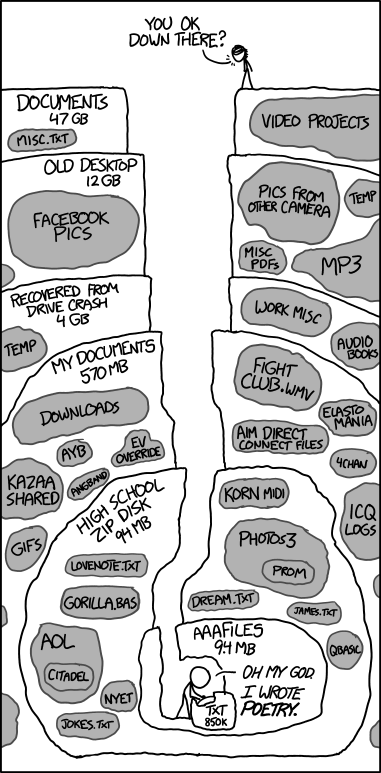
\includegraphics[width=\linewidth]{./gfx/14-xkcd-old-files}
%
\column{.5\linewidth}
\begin{center}
\emph{Wow, ANIMORPHS-NOVEL.RTF? Just gonna, uh, go through and delete that from all my archives real quick.}

\vspace{12pt}
Source: \url{https://xkcd.com/1360/}
\end{center}
\end{columns}
%
\end{frame}

% =========================================================================== %

\begin{frame}{Thinking About File Systems}
%
\begin{center}
	\includegraphics[width=.8\linewidth, page=1]{./gfx/14-filesystems}
\end{center}
%
\end{frame}

% =========================================================================== %

\begin{frame}{Structure Elements of a Partition}
%
\begin{columns}[T]
\column{.65\linewidth}
	% trim = left bottom right top
	\includegraphics[width=\linewidth, page=2, trim = 0 70 0 30]{./gfx/14-filesystems}
	
	\scriptsize
	The terminology used here is specific to the ext file systems used in linux systems. The core ideas, however, also apply to FAT, NTFS (Windows) and HFS/HFS+/APFS/MFS (MacOS).
%
\column{.3\linewidth}
	\small
	\begin{itemize}
	\item There can be multiple file systems (partitions) on a single physical device.
	\item There are dozens of file systems, all with their particular inner workings
	\item Most important differences between file systems: access management, fail safes, compression options
	\end{itemize}
\end{columns}
%
\end{frame}

% =========================================================================== %

\begin{frame}{Regular Files and Fragmentation}
%
\vspace{-3pt}
\begin{center}
% trim = left bottom right top
\includegraphics[width=.95\linewidth, page=3,trim=0 300 0 20,clip]{./gfx/14-filesystems}
\end{center}

\vspace{-3pt}
\begin{columns}
\column{.5\linewidth}
	\begin{itemize}
	\item List of entries: tuples of strings and inodes
	\item Inodes: Metadata and actual location: cluster ID
	\end{itemize}
%
\column{.5\linewidth}
	\begin{itemize}
	\item Blocks/Clusters: fixed size
	\item Larger files: multiple clusters
	\item[\Thus] Fragmentation
	\end{itemize}
\end{columns}
%
\end{frame}

% =========================================================================== %

\begin{frame}{Hardlinks}
%
\vspace{-3pt}
\begin{center}
% trim = left bottom right top
\includegraphics[width=.95\linewidth, page=4,trim=0 300 0 20,clip]{./gfx/14-filesystems}
\end{center}
%
\vspace{-6pt}
\begin{columns}
\column{.5\linewidth}
	\begin{itemize}
	\item Multiple entries in List of Entries can point to same inode
	\item[\Thus] Same file in two (or more) locations
	\item Changes affect both locations
	\end{itemize}
%
\column{.5\linewidth}
	\begin{itemize}
	\item Imagine shared ressource for several project folders
	\item File is only deleted when all references are removed
	\end{itemize}
\end{columns}
%
\end{frame}

% =========================================================================== %

\begin{frame}{Tangent: No Hard Links to Directories}
%
\begin{columns}
\column{.6\linewidth}
\begin{itemize}
\item Directories are modelled in inodes, too
\item In principle: possible to create a hardlink to a directory
\item But this would allow circular references!
	\begin{itemize}
	\item Imagine subdirectories \texttt{root/foo}
	\item Create a hardlink \texttt{bar} under \texttt{foo} linking to \texttt{root}
	\item Now write a program that recursively lists all subdirectories of \texttt{root}
	\item[\Thus] Possible, but will give you a headdache every time you touch files
	\item[\Thus] Forbidden!
	\end{itemize}
\item Exceptions
	\begin{itemize}
	\item \texttt{.} is a hardlink to the the directory itself
	\item \texttt{..} is a hardlink to the parent directory
	\end{itemize}
\end{itemize}
%
\column{.4\linewidth}
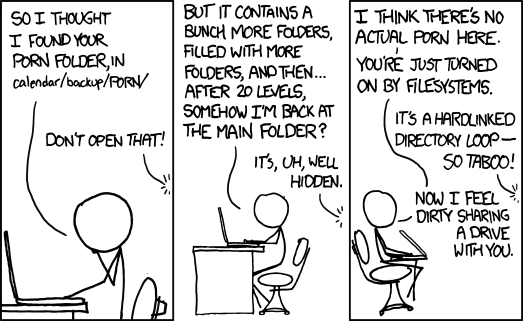
\includegraphics[width=\linewidth]{./gfx/14-xkcd-porn-folder}
\vspace{3pt}
\scriptsize
\emph{Eww, gross, you modified link()? How could you enjoy abusing a filesystem like that?}

\vspace{9pt}
Source: \url{https://xkcd.com/981/}
\end{columns}
%
\end{frame}

% =========================================================================== %

\begin{frame}{Symbolic Links (aka SymLinks)}
%
\vspace{-6pt}
\begin{center}
% trim = left bottom right top
\includegraphics[width=.95\linewidth, page=5,trim=0 300 0 20,clip]{./gfx/14-filesystems}
\end{center}
%
\vspace{-12pt}
\begin{columns}
\column{.5\linewidth}
	\begin{itemize}
	\item Speical kind of inode
	\item Content: referenced file
	\item In principle same effect
	\end{itemize}
%
\column{.5\linewidth}
	\begin{itemize}
	\item Moving/Deleting original file breaks link
	\item Works with folders and across file systems
	\end{itemize}
\end{columns}
%
\end{frame}

% =========================================================================== %

\begin{frame}{Link Files}
%
% trim = left bottom right top
\includegraphics[width=\linewidth, page=6,trim=0 300 0 20,clip]{./gfx/14-filesystems}
%
\begin{columns}
\column{.5\linewidth}
	\begin{itemize}
	\item Like SymLinks, but done in regular files
	\item Treated by GUI rather than OS
	\item Same (dis)advantages
	\end{itemize}
%
\column{.5\linewidth}
	\begin{itemize}
	\item Windows: \texttt{.lnk} files
	\item Linux: \texttt{.desktop} files
	\item Mac: I don't have a fucking clue
	\end{itemize}
\end{columns}
%
\end{frame}

% =========================================================================== %

\begin{frame}
%
\begin{columns}
\column{.5\linewidth}
\begin{hintbox}[Following Symlinks and Link Files]
	\footnotesize
	Not all programs automatically follow symlinks. \emph{Most} programs don't follow \emph{link files}. One example is a zip program I was using in uni, to the effect
	that I nearly failed a course.
	
	\vspace{3pt}
	You can find out about the nature by visual clues: in Windows, link files and symlinks are rendered with an arrow in the lower left corner.
	Depending on your file browser, symlinks sometimes are rendered in different colours.
	
	\vspace{3pt}
	In the console, \texttt{ls -l} (Linux/Mac) or \texttt{dir /a} (Windows) reveals the true nature of a file.
\end{hintbox}
%
\column{.5\linewidth}
	\begin{center}
		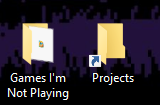
\includegraphics[width=.4\linewidth]{./gfx/14-link-folder}
	\end{center}
	
	\begin{center}
		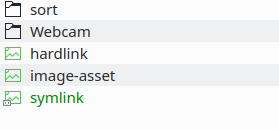
\includegraphics[width=.8\linewidth]{./gfx/14-link-linux}
	\end{center}
	
	\begin{center}
		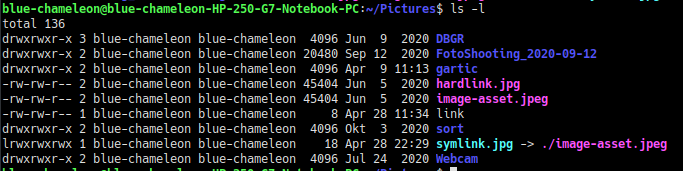
\includegraphics[width=1.\linewidth]{./gfx/14-link-terminal}
	\end{center}
	
	
\end{columns}
%
\end{frame}

% =========================================================================== %

\begin{frame}{OS API: A New Layer of Problems}
%
\begin{itemize}
\item Most of what we've just seen: hidden away in OS API calls\footnote{We can create hardlinks and symlinks easily, but will usually never touch inodes directly.}
\item OS provides a \emph{layer of abstraction} that is meant to reduce complex operations to easy string manipulation
	\begin{itemize}
	\item Problem 1: multiple OS'es with different conventions
	\item Problem 2: tedious to implement the same string operations again and again
	\end{itemize}
\item[\Thus] \texttt{pathlib}: Uniform abstraction layer, allowing OS-agnostic access to the file system
	\begin{itemize}
	\item Pure String-Level operations like \emph{extract the file name from \texttt{/foo/bar/somefile.txt}}
	\item True file system operations like \emph{list all files under \texttt{/foo/bar}}
	\end{itemize}
\end{itemize}
%
\end{frame}

% =========================================================================== %

\begin{frame}[fragile]{Tangent: POSIX}
%
\begin{itemize}
\item POSIX: Portable Operation System Interface
	\begin{itemize}
	\item Standard, published and maintained by the IEEE
	\item Defines APIs for low level OS operations, behaviour of shells, available shells, ...
	\item Examples: Threading library \texttt{pthread}, commands like \texttt{gcc}, \texttt{grep}, \texttt{awk}, ...
	\item Organized into volumnes, \zB \emph{POSIX.10: Directory Structure and Devices}
	\item Check out: \url{https://www.open-std.org/jtc1/sc22/open/n4217.pdf} (3718 pages)
	\end{itemize}
\item[\Thus] Meant to make life easier
	\begin{itemize}
	\item Source code should act the same when deployed on different, POSIX-compliant OS'es
	\item MacOS: fully compliant since V10.5 (Leopard)
	\item Windows: partially compliant at best
		\begin{itemize}
		\item POSIX subsystem 1993-2003, SFU (services for unix) until 2012; WSL since 2016
		\item Cygwin, MinGW, etc.: third party tools
		\end{itemize}
	\item Linux: \emph{mostly compliant}
		\begin{itemize}
		\item GNU often requires environment variables like \texttt{POSIXLY\_CORRECT}\footnote{%
			formerly \texttt{POSIX\_ME\_HARDER}
		} to be set
		\end{itemize}
	\end{itemize}
\end{itemize}
%
\end{frame}

% =========================================================================== %

\begin{frame}{Pathlib Architecture}
%
\begin{columns}
\column{.5\linewidth}
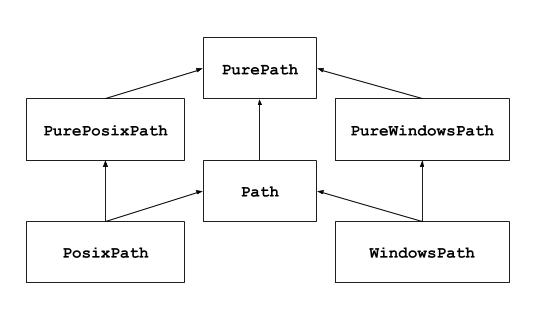
\includegraphics[width=\linewidth]{./gfx/14-pathlib-inheritance}
%
\begin{hintbox}[Genealogy of \texttt{pathlib}]
\scriptsize 
The \texttt{pathlib} is built on top of the python modules \texttt{os}, \texttt{posixpath}, \texttt{ntpath}, \texttt{fnmatch}, \texttt{re}, \texttt{functools}, \texttt{io} and \texttt{sys}.
\end{hintbox}
%
\column{.5\linewidth}
\begin{itemize}
\item Principal object: Instances of \texttt{pathlib.Path}
	\begin{itemize}
	\item Automatically evolves into \texttt{PosixPath} on unixoid systems or from \texttt{WindowsPath} on Windows
	\item The \texttt{Pure...Path} variations provide String level manipulations
	\item Their child classes can also access the real file system
	\item Instantiation of \texttt{Pure...Path}s possible regardless of active OS
	\item The concrete \texttt{Path} variants are only available on the corresponding OS'es
	\end{itemize}
\end{itemize}
\end{columns}
%
\end{frame}

% =========================================================================== %

\begin{frame}[fragile]{Construction of Paths}
%
\begin{itemize}
\item Via Constructor
	\begin{itemize}
	\item \texttt{Path(someString)} -- dissects \texttt{someString} into its elements (drive, directories, file name) according to OS convention
	\item \texttt{Path(*iterable)} -- dissects each element of \texttt{iterable} separately, then joins the parts to a full path.
		\begin{itemize}
		\item \inPy{Path("foo", "bar")} becomes \inPy{...Path('foo/bar')}
		\item \inPy{Path("foo", "/bar")} becomes \inPy{...Path('/bar')}
		\item The elements of \texttt{iterable} may be \inPy{str}ings or instances of \inPy{PurePath}, too
		\end{itemize}
	\item \texttt{PureWindowsPath} treats both, \texttt{/} and \texttt{\textbackslash} as directory separators
	\item \texttt{PurePosixPath} only accepts \texttt{/} as directory separator\footnote{%
		It \emph{is} possible to create a file named \texttt{\textbackslash foo}. That you can does not mean that you should, though...
	}
	\end{itemize}
\item Via \texttt{joinpath} method
	\begin{itemize}
	\item \inPy{pathInstance = Path("foo")}
	\item \inPy{pathInstance.joinpath("bar")} gives \inPy{...Path('foo/bar')}
	\item Shorthand version: \inPy{pathInstance / "bar"}
	\item Also: \texttt{pathInstance / otherPathInstance} (and likewise with \texttt{pathjoin)}
	\end{itemize}
\end{itemize}
%
\end{frame}

% =========================================================================== %

\begin{frame}{Dissecting Paths (I)}
%
\begin{itemize}
\item \texttt{instance.parts} gives a \inPy{tuple} of the \emph{atoms} of the path
	\begin{itemize}
	\item \texttt{PureWindowsPath("C:/foo/bar").parts} gives \inPy{('C:\\', 'foo', 'bar')}
	\end{itemize}
\item \texttt{instance.parent} gives a Path comprising all but the last segment
	\begin{itemize}
	\item \inPy{Path("/a/b/c/d/").parent} gives \inPy{...Path('/a/b/c')}
	\item \inPy{Path("/").parent} gives \inPy{...Path('/')}
	\end{itemize}
\item \texttt{instance.parents} gives an immuatable sequence parent Paths
	\begin{itemize}
	\item \inPy{PureWindowsPath("C:/foo/bar").parents[0]} gives \inPy{PureWindowsPath("C:\\foo\\")}
	\item \inPy{PureWindowsPath("C:/foo/bar").parents[1]} gives \inPy{PureWindowsPath("C:\\")}
	\end{itemize}
\item \texttt{instance.anchor} gives the root element of a Path
	\begin{itemize}
	\item \inPy{PureWindowsPath("C:/foo/bar").anchor} gives \inPy{'C:\\'}
	\item \inPy{PurePosixPath("/foo/bar").anchor} gives \inPy{'/'}
	\end{itemize}
\end{itemize}
%
\end{frame}

% =========================================================================== %

\begin{frame}{Dissecting Paths (II)}
%
\begin{itemize}
\item \texttt{instance.name} gives \emph{the last segment of a Path, excluding the drive}
	\begin{itemize}
	\item \inPy{PureWindowsPath("C:/foo/bar").name} gives \inPy{'bar'}
	\item \inPy{PureWindowsPath("C:/").name} gives \inPy{''}
	\item Usually a file name, but could also be a directory
	\end{itemize}
\item \texttt{instance.suffix} gives the \emph{part of the name after the last dot}
	\begin{itemize}
	\item \inPy{Path("foo/bar.ext").suffix} gives \inPy{'ext'}
	\item \inPy{Path("foo/bar.tar.gz").suffix} gives \inPy{'gz'}
	\item \inPy{Path("foo/bar").suffix} gives \inPy{''}
	\item Again, no special treatment of directories
	\end{itemize}
\item \texttt{instance.suffixes} a list of all things that look like an extension
	\begin{itemize}
	\item \inPy{Path("foo/bar.tar.gz").suffixex} gives \inPy{['tar', 'gz']}
	\end{itemize}
\item \texttt{instance.stem} gives \texttt{.name} without the \texttt{.suffix} part
	\begin{itemize}
	\item \inPy{Path("foo/bar.ext").stem} gives \inPy{'bar'}
	\item \inPy{Path("foo/bar.tar.gz").stem} gives \inPy{'bar.tar'}
	\end{itemize}
\end{itemize}
%
\end{frame}

% =========================================================================== %

\begin{frame}{Back To Strings}
%
\begin{itemize}
\item \inPy{str(instance)} Usually does the job
	\begin{itemize}
	\item Uses the native conventions concerning path separator
	\item \inPy{str(PureWindowsPath("C:/foo/bar"))} gives \inPy{'C:\\foo\\bar'}
	\item \inPy{str(PurePoxixPath("/foo/bar"))} gives \inPy{'/foo/bar'}
	\end{itemize}
\item \texttt{instance.as\_posix()} always uses forward slashes (/)
	\begin{itemize}
	\item \inPy{PureWindowsPath("C:/foo/bar").as_posix} gives \inPy{'C:/foo/bar'}
	\item \inPy{PurePoxixPath("/foo/bar").as_posix} gives \inPy{'/foo/bar'}
	\end{itemize}
\item \texttt{instance.as\_uri()} renders the Path as an \emph{unique ressource identifier}
	\begin{itemize}
	\item The Path must be absolute
	\item A \inPy{ValueError} is raised, if it is not absolute
	\item \inPy{PureWindowsPath("C:/foo").as_uri} gives \inPy{'file:///C:/foo/bar'}
	\item \inPy{PurePoxixPath("/foo/").as_uri} gives \inPy{'file:///foo'}
	\item \inPy{PurePoxixPath("foo/").as_uri} raises a \inPy{ValueError}.
	\end{itemize}
\end{itemize}
%
\end{frame}

% =========================================================================== %

\begin{frame}[fragile]{Relative and Absolute Paths (I)}
%
\begin{itemize}
\item \texttt{instance.is\_absolute()} returns a \inPy{bool}ean based the first Path segment
\item \texttt{is\_relative\_to(*other)} returns a \inPy{bool}ean telling wehter \texttt{other} is a child of \texttt{instance}.
	\begin{itemize}
	\item This does not resolve references to current or parent directory (\texttt{.} and \texttt{..})
	\item \inPy{Path("foo/bar/../baz").is_relative_to("foo")} is \inPy{True}
	\item \inPy{Path("foo/").is_relative_to("foo")} is \inPy{True}
	\item \inPy{Path("foo/bar/../baz").is_relative_to("foo/baz")} is \inPy{False}\footnote{%
		We'll see very soon how to normalize paths.	
	}
	\end{itemize}
\item \texttt{instance.relative\_to(*other)} constructs a relative Path, if possible
	\begin{itemize}
	\item \inPy{Path("foo/bar").relative_to("foo")} gives \inPy{...Path('bar')}
	\item \inPy{Path("/foo/bar").relative_to("foo")} raises a \inPy{ValueError} (not both Paths absolute)
	\item \inPy{Path("/foo/bar").relative_to("/baz")} raises a \inPy{ValueError} (no common root)
	\end{itemize}
\end{itemize}
%
\end{frame}

% =========================================================================== %

\begin{frame}[fragile]{Relative and Absolute Paths (II)}
%
\begin{defbox}[Concrete Paths ahead]
\scriptsize
All previously mentioned attributes and methods acted on \texttt{PurePath}s. The following methods require concrete \texttt{Path}s.
\end{defbox}
%
\begin{itemize}
\item \texttt{instance.absolute()} returns a \texttt{Path} representing an absolute location
	\begin{itemize}
	\item Assumed to be relative to the CWD
	\item Does not resolve symlinks or parent directory segments (\texttt{..})
	\item \inPy{Path(".").absolute()} gives \inPy{...Path('/home/yourUserName')}
	\item \inPy{Path("..").absolute()} gives \inPy{...Path('/home/yourUserName/..')}
	\end{itemize}
\item \inPy{instance.resolve(strict=False)} returns a normalized version of \texttt{.absolute()}
	\begin{itemize}
	\item Symlinks and parent directory segments (\texttt{..}) are resolved
	\item If \inPy{strict=True}, existence of path is checked: throws \inPy{FileNotFoundError} if no such file or folder exists
	\item \inPy{Path("..").resolve()} gives \inPy{...Path('/home')}
	\item \inPy{Path("symlink/foo").resolve()} gives \inPy{...Path('/target/foo')}
	\end{itemize}
\end{itemize}
%
\end{frame}

% =========================================================================== %

\begin{frame}[fragile]{Special Folders}
%
\begin{hintbox}[Tilde Symbol (\textasciitilde)]
\scriptsize
On unixoid systems, the tilde symbol (\texttt{\textasciitilde}) is a shorthand for the home directory of the current user.\\
The Stringn \texttt{\textasciitilde <user>} is replaced by the home directory of user \texttt{<user>}.
\end{hintbox}
%
\begin{itemize}
\item \texttt{instance.expanduser()} replaces \texttt{\textasciitilde} and \texttt{\textasciitilde <user>} by the proper home directory
	\begin{itemize}
	\item Also works on Windows
	\item \inPy{Path("~myColleague/projects").expanduser()} returns \inPy{Path('/home/myColleague/projects')}
	\end{itemize}
\item \texttt{Path.home()} the current user's home directory
	\begin{itemize}
	\item Class method
	\item Simply a better readable shortcut to \inPy{Path("~").expanduser()}
	\end{itemize}
\item \texttt{Path.cwd()} the current working directory
	\begin{itemize}
	\item Class method
	\item Simply a better readable shortcut to \inPy{Path(".").absolute()}
	\end{itemize}
\end{itemize}
%
\end{frame}

% =========================================================================== %

\begin{frame}[fragile]{Probing File System Character}
%
\begin{itemize}
\item \texttt{instance.exists()} returns a \inPy{bool}ean telling whether \texttt{instance} exists
	\begin{itemize}
	\item If \texttt{instance} describes a symlink, the existence of the target is tested.
	\item Use \texttt{instance.is\_symlink()} to test for existing broken symlinks
	\end{itemize}
\item \texttt{instance.is\_file()} returns a \inPy{bool}ean telling whether \texttt{instance} is a regular file or a symlink to a file
\item \texttt{instance.is\_dir()} returns a \inPy{bool}ean telling whether \texttt{instance} is a directory or a symlink to a directory
\item \texttt{instance.is\_symlink()} returns a \inPy{bool}ean telling whether \texttt{instance} is a symlink, whether broken or not
\item \texttt{instance.readlink()} returns the target of a symlink
\end{itemize}
%
\begin{hintbox}[There's more]
\scriptsize
The unix philosophy \emph{Everything is a file} allows to treat hardware like keyboard, abstract entities like the shell and other things as files, too.
See \url{https://docs.python.org/3/library/pathlib.html} for more functions.
\end{hintbox}
%
\end{frame}

% =========================================================================== %

\begin{frame}[fragile]{Tangent: Opening a Broken Symlink}
%
\begin{itemize}
\item Assume a symlink \texttt{link.dat} exists and refers to \texttt{target.dat}
\item But \texttt{target.dat} does not exist (was deleted)
\item In Python...
	\begin{itemize}
	\item \inPy{open("link.dat", "r")} causes a \inPy{FileNotFoundError}
	\item \inPy{open("link.dat", "w")} creates a new file \texttt{target.dat}
	\end{itemize}
\item[\Thus] Simply checking \texttt{pathInstance.exists()} before write operations is usually sufficient to prevent data loss.
\item[\Thus] Use these to identify broken symlink and check any name for existence:
	\begin{minted}[fontsize=\footnotesize]{python3}
def is_broken_symlink(path):
    return path.is_symlink() and not path.exists()
    
def exists_extended(path):
    return path.is_symlink() or path.exists()
	\end{minted}
\end{itemize}
%
\end{frame}

% =========================================================================== %

\begin{frame}[fragile]{Listing Existing File System Entities (I)}
%
\begin{itemize}
\item \texttt{instance.iterdir()} returns an iterator over the contents of \texttt{instance}
	\begin{itemize}
	\item Assumes \texttt{instance} describes a directory
	\item No recursive traversal of the directory behind \texttt{instance}
	\item If \texttt{instance} is not a directory, \texttt{instance.iterdir()}  still returns a generator object, but calling \inPy{next} on it raises a \inPy{NotADirectoryError}
	\end{itemize}
\item \texttt{instance.glob(pattern)} returns an iterator over the contents of \texttt{instance} \emph{that match \texttt{pattern}}
	\begin{itemize}
	\item Pattern is a \inPy{str}ing that may contain wildcards
	\item \texttt{?} -- an arbitrary character
	\item \texttt{*} -- zero or more arbitrary characters
	\item \texttt{**/} -- an arbitrary subfolder structure
	\item \texttt{[chars]} -- any of the characters in \texttt{chars}
	\item \texttt{[!chars]} -- none of the characters in \texttt{chars}
	\item Python 3.11 or newer: if \texttt{pattern} ends in \texttt{/}, only directories are listed
	\end{itemize}
\end{itemize}
%
\end{frame}

% =========================================================================== %

\begin{frame}[fragile]{Listing Existing File System Entities (II)}
%
\begin{itemize}
\item \texttt{instance.rglob(pattern)} like \texttt{glob}, but automatically adds \texttt{**/} to \texttt{pattern}
\item Examples
	\begin{itemize}
	\item List all JPEG files that do not start with a or A and are stored in \texttt{./pictures} or its subdirectories\\
		\inPy{Path("pictures").glob("**/[!aA]*.jpg")} or \\
		\inPy{Path("pictures").rglob("[!aA]*.jpg")}
	\item List all directories that start with a \texttt{t} \\
		\inPy{Path().glob("**/t*/")} or \\
		\inPy{Path().rglob("t*/")}
	\end{itemize}
\end{itemize}
%
\begin{hintbox}[Lazy Evaluation]
\scriptsize
\texttt{iterdir}, \texttt{glob} and \texttt{rglob} only return iterators. The actual traversal of the file system happens lazily, \ie only when you invoke \texttt{list(...glob())} or the like.
\end{hintbox}
%
\end{frame}

% =========================================================================== %

\begin{frame}[fragile]{Creating Files, Directories and Links}
%
\begin{itemize}
\item \inPy{instance.touch(mode=0o666, exist_ok=True)} creates a new empty file
	\begin{itemize}
	\item \texttt{mode} refers to the \emph{ACL} (Access Control List) -- See next Slide
	\item \texttt{exists\_ok} controls what happens when \texttt{instance.exists()}
		\begin{itemize}
		\item Do nothing if \inPy{True}
		\item Raise \inPy{FileExistsError} Otherwise
		\end{itemize}
	\end{itemize}
\item \inPy{instance.mkdir(mode=0o777, parents=False, exist_ok=False)} creates a new empty directory
	\begin{itemize}
	\item \texttt{mode} and \texttt{exit\_ok} have the same meaning as with \texttt{touch}
	\item \texttt{parents} controls what happens when \texttt{instance.parent} does not exist
		\begin{itemize}
		\item If \inPy{True}, all missing directories are created, too
		\item Otherwise, raises a \inPy{FileNotFoundError}
		\end{itemize}
	\end{itemize}
\item \inPy{instance.symlink_to(target, target_is_directory=False)} makes \texttt{instance} a symlink to \texttt{target}
	\begin{itemize}
	\item \texttt{target\_is\_directory} must be set correctly under Windows and is ignored under unixoid systems
	\end{itemize}
\item \texttt{instance.hardlink\_to(target)} makes \texttt{instance} a hardlink to \texttt{target}
\end{itemize}
%
\end{frame}

% =========================================================================== %

\begin{frame}{Tangent: Access Control Lists (ACLs)}
%
\begin{itemize}
\item Idea: Different users should have different levels of permission on a \emph{per file level}
	\begin{itemize}
	\item Admins should be able to do anything
	\item Some files should be read-only to some users
	\item Kinds of permissions specific to the various file systems; here: POSIX-ACLs
	\end{itemize}
\item Kinds of access
	\begin{itemize}
	\item Read, Write, Execute (files) or allow traversal (directories)
	\item Represented by an integer 4, 2, and 1, respectively
	\item[\Thus] Sum/Logical Or of the flags tells what you can do with the file
	\end{itemize}
\item Multiple Instances of these access restrictions:
	\begin{itemize}
	\item File Owner (the one who created the file)
	\item File Group (users can be members of multiple groups)
	\item World (everyone with access to the drive)
	\end{itemize}
\item[\Thus] Three digit octal number, \texttt{0oOGW}
	\begin{itemize}
	\item Try in terminal \texttt{ls -l}, see column like \texttt{-rw-rw-r-{}-}
	\item First \enquote{digit} encodes type (here regular file; also \texttt{d} for directory)
	\item Read/Write access for owner and group, read-access for world
	\end{itemize}
\end{itemize}
%
\end{frame}

% =========================================================================== %

\begin{frame}[fragile]{Changing ACLs After Creation}
%
\begin{itemize}
\item \inPy{instantce.chmod(mode, *, follow_symlinks=True)} -- changes the access bits of \texttt{instance} to \texttt{mode}
	\begin{itemize}
	\item If \inPy{follow_symlinks = False}, the ACL bits of the link are changed rather than those of the target
	\end{itemize}
\item \texttt{instance.lchmod(mode)} -- same as \inPy{instantce.chmod(mode, follow_symlinks=False)}
\item \texttt{instance.owner()} and \texttt{instance.group()} reveal the owner and group of a file (\emph{read-access} only)
\item \texttt{instance.stat()} returns an \texttt{os.stat\_result} object. 
	(See \href{https://docs.python.org/3/library/os.html#os.stat_result}{\thus \emph{the docs}})
\end{itemize}
%
\begin{hintbox}[Terminal Commands]
\scriptsize
The POSIX command line tool \texttt{chmod} achieves the same goal. You can also type commands like \texttt{chmod +x file} to add execution rights or \texttt{chmod -w file} to remove write access.

\vspace{3pt}
Further, there's \texttt{chown} (changes the owner of a file) and \texttt{chgrp} (changes the group to which a file belongs).
\end{hintbox}
%
\end{frame}

% =========================================================================== %

\begin{frame}{Moving and Removing Files and Directories}
%
\begin{itemize}
\item \texttt{instance.rename(target)} renames a file or directory.
	\begin{itemize}
	\item \texttt{target} may be anything from which a \texttt{Path} can be constructed \\
		(most often simply a String)
	\item If \texttt{target} points to a different directory than the current location of \texttt{instance}, the file/directory is moved
	\item Returns the new \texttt{target}
	\item If \texttt{target} already exists...
		\begin{itemize}
		\item Windows: raises an \inPy{FileExistsError}
		\item Unix: overwrites the existing File!
		\end{itemize}
	\end{itemize}
\item \inPy{instance.unlink(missing_ok=False)} removes hardlink/symlink or deletes file
	\begin{itemize}
	\item If \inPy{missing_ok == False} and \texttt{instance} does not exist, raises \inPy{FileNotFoundError}
	\item If \texttt{instance} refers to a directory, raises \inPy{IsADirectoryError}
	\end{itemize}
\item \texttt{instance.rmdir()} removes an \emph{empty} directory.
	\begin{itemize}
	\item Raises \inPy{NotADirectoryError} if not a directory
	\item Raises \inPy{OSError} if not empty
	\end{itemize}
\end{itemize}
%
\end{frame}

% =========================================================================== %

\begin{frame}
%
\vspace{-16pt}
\begin{center}
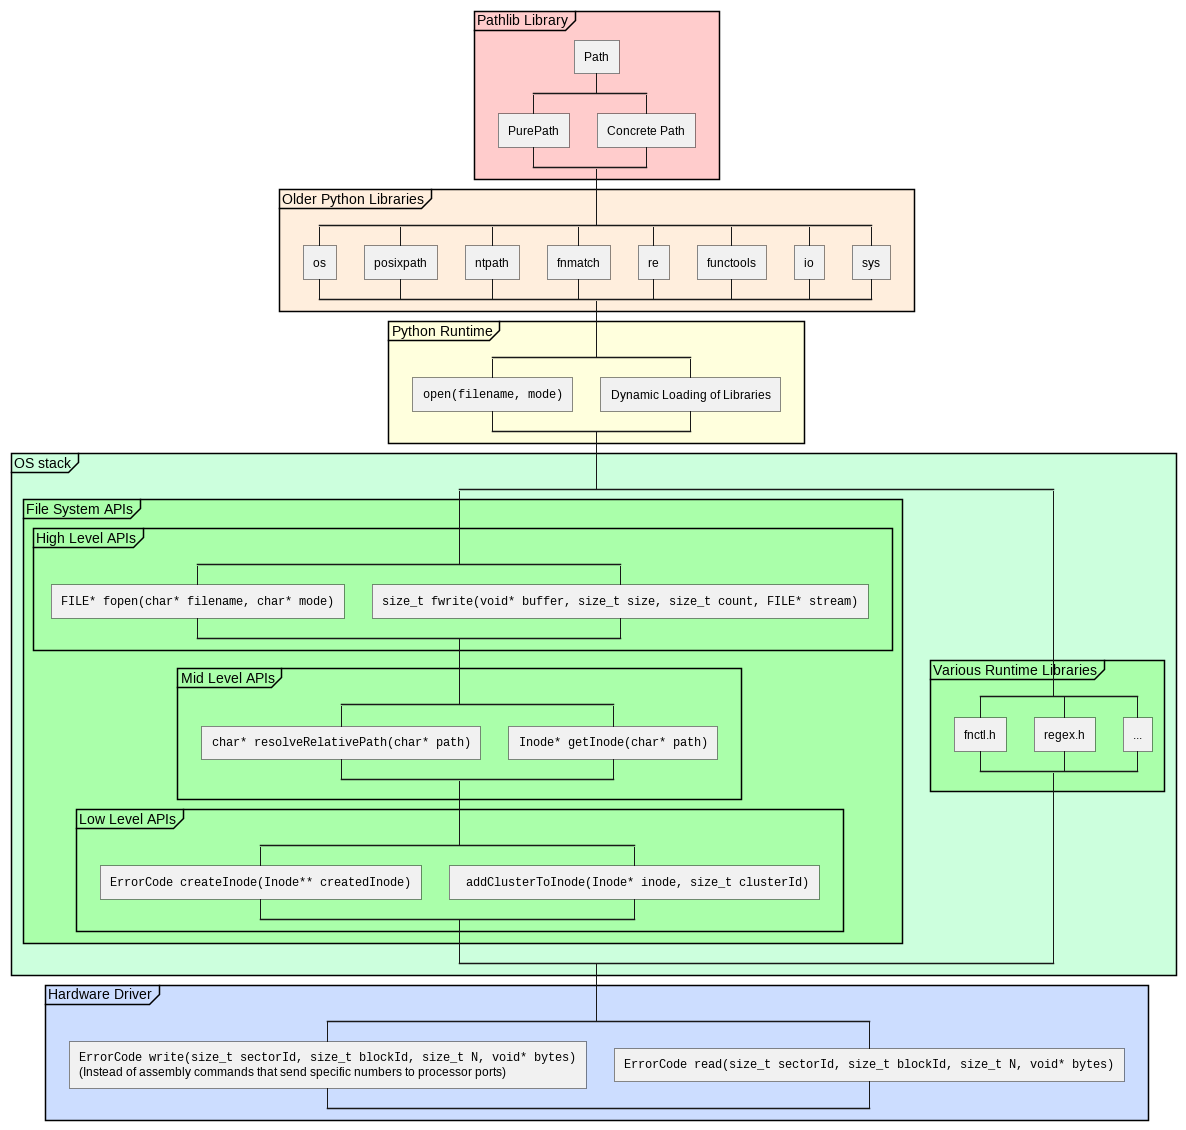
\includegraphics[width=.66\linewidth]{./gfx/14-pathlib-stack}
\end{center}
%
\end{frame}

% =========================================================================== %
\end{document}

% MAREI!!
% whom do I give credit? Where?